%\title{ACTUAL MASTER LAB DOCUMENT}
%This is the original Master Lab Document template, from this the COPY THIS Master Lab Document is created which then can be copied easily to create new labs.
\documentclass{article}
\usepackage[utf8]{inputenc}
\usepackage{cccu_lab}

\modulecode{MCOMD3AOS}
\labtitle{System Statistics Shell Script}
\author{Sebastian Blair}
\date{\today}

\begin{document}
\begin{titlepage}
\makeatletter
\vspace*{5cm}
\begin{center}
\textcolor{Periwinkle}{ % Red font color
		{\Huge \@modulecode}\\[0.5\baselineskip] % Title line 1
		{\Large ---}\\[0.5\baselineskip] % Title line 2
		{\Huge \@labtitle} % Title line 3
}
\end{center}
\rule{\textwidth}{1pt} \\

\begin{center}
\begin{tabular}{r|l}
Author & \textbf{\@author} \\
Last Update & \textbf{\@date} \\
Number of pages & \textbf{\pageref{LastPage}}
\end{tabular}
\end{center}
\centering
\vspace{3em}
\vfill
Environmental Impact Per Page $\approx$ $10.2\unit{L}$ water, $2\unit{g}$ CO$_{2}$ and $2\unit{g}$ wood. 
\vspace{2em}

The environmental effects of paper production include deforestation, the use of enormous amounts of energy and water as well as air pollution and waste problems. Paper accounts for around 26\% of total waste at landfills

\vspace{2em}

Therefore, please print only if this is really necessary.


\end{titlepage}
\makeatother


\section*{Content}
\label{sec:content}

\begin{table}[H]
    \centering
    \begin{tabular}{c|c}
        \nameref{sec:intro}           & ~ \\ % the ~ is just a placeholder in a table that prints nothing but fills the cell anyway; good for making sure everything is aligned properly
        \nameref{sec:globalVariables} & ~ \\
        \nameref{sec:errorChecking}   & ~ \\
        \nameref{sec:usageFunction}   & ~ \\
        \nameref{sec:theArguments}    & ~ \\
    \end{tabular}
\end{table}

\section*{Introduction}
\label{sec:intro}

So like last week we are going to keep adding to our \code{usage.sh} script we created using \code{bash} on JupyterHub. 

\begin{shaded}
\textbf{\faInfo} \hspace{1em} NOTICE
Jupyterhub link here:
\begin{itemize}
    \item \url{https://jupyterhub.canterbury.ac.uk/}
    \item Sign in with your CCCU Microsoft account.
    \item In launcher menu click Terminal and Bash
    \item Once in terminal mode, either make a directory (\code{mkdir}) called `AOS' or navigate to it if you did this last time (\code{cd}). 
    \item Now create a file called \code{systemStats.sh} with by writing into the terminal \code{nano systemsStats.sh}, if you already have a \code{usage.sh} from last week do the following \code{mv usage.sh systemStats.sh} and then \code{nano systemStats.sh}. 
\end{itemize}
\end{shaded}

\section{Front Matter}
\label{sec:frontMatter}
Once completed the script should output the following information to the terminal, as seen in \cref{fig:outputofscript}.

% FIXME: Replace figure with a more legible version (font issue in screenshot)
\begin{figure}[H]
    \centering
    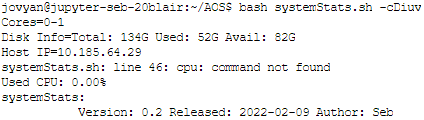
\includegraphics[width=1\textwidth]{images/systemStats_output.PNG}
    \caption{Output of script}
    \label{fig:outputofscript}
\end{figure}

First of make sure your file looks like code shown below.

\inputminted[frame=single,firstline=1, lastline=5,linenos]{bash}{./systemStats.sh}

In shell scripting comments, where the compiler ignores these lines, is defined as \code{\#}. The first line is special it points to the directive of the interpreter for the scripting language you are using, in this case bash. We call the \code{\#!} a hash-bang, shebang, hash-pling etc. The idea is it makes the shell script more like an executable file.

\begin{center}
\vspace{5em}
    Intentionally left blank, continues overleaf\ldots
\end{center}

\section{Global Variables}
\label{sec:globalVariables}
Next we are going to define some \code{global} variables, in bash all variables are \code{global} unless you specify that they are \code{local}.

\inputminted[frame=single,firstline=6, lastline=8,linenos]{bash}{./systemStats.sh}

Remember that bash is very particular language and whitespaces mean something.  So make sure that variable for example have no spaces. We are going to use these variables later when we call for the version information of the script.

\section{Usage function}
\label{sec:usageFunction}
Now we are going to write a function that when called will display a help message on the terminal about the script, as example see below. 

\begin{figure}[H]
    \centering
    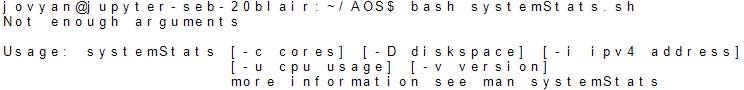
\includegraphics[width=1\textwidth]{images/systemStats_output_usage.PNG}
    \label{fig:my_label}
\end{figure}

To do this we need to write the following code\ldots

\inputminted[frame=single,firstline=10, lastline=16,linenos]{bash}{./systemStats.sh}

Similarly our function name is in upper case as this is global too on line 110. The subsequent lines use the \code{echo} command with to output information to standard out, or in this case the terminal. When supplied with the argument \code{-e} we enable the use of escape character such as; 
\begin{itemize}
    \item \code{\textbackslash n} new line
    \item \code{\textbackslash t} tab identation 
\end{itemize}

Line 12, \code{\$1} means first argument passed into this function. The following lines will print out on a new line every time the content in side the \code{""}. This information will tell the user of the script what arguments the script takes and the arguments descriptions.

\begin{center}
\vspace{8em}
    Intentionally left blank, continues overleaf\ldots
    \vspace{2em}
\end{center}

\section{Error Checking}
\label{sec:errorChecking}
Next we are going to some basic error checking.

\inputminted[frame=single,firstline=17, lastline=27,linenos]{bash}{./systemStats.sh}

Conditional checks can be performed in many styles within bash, here we see two styles.

Firstly, like we see on lines 18 and 21, \code{[ ]} is the same as a \code{built-ins} \code{test} command. It supports single conditional checks, and subsequent checks must be performed in separate brackets, separated by Boolean operators, \code{\& \&} and \code{||} and doesn't support the \code{!} NOT operator. To invert a condition, use a ! outside the first bracket to use the shell's facility for inverting command return values.

Secondly, line 24, \code{[[ ]]} is a bash is bash-specific, though others shells may have implemented similar constructs. The operators \code{==} and \code{!=} apply bash pattern matching rules, see "Pattern Matching" in man bash has a \code{=\textasciitilde} regex match operator allows use of parentheses and the \code{!}, \code{\&\&}, and \code{||} logical operators within the brackets to combine subexpressions.

So back to lines 18 and 21 check to see if the length of arguments, \code{\$\#}, is less than, \code{-lt} and a separate check for greater than, \code{-gt}.

Line 24, shows we are checking for a match in patterns that are not numeric. So the conditional check is comparative to see it \code{\$1} matches either \code{-h} or \code{'--help'}.

Also, notice how we are using \code{exit 1}, which indicates an error. 

\begin{shaded}
\textbf{\faSpaceShuttle} \hspace{1em} WOULD YOU LIKE TO KNOW MORE\ldots ?
\begin{itemize}
    \item Exit code 0  \hspace{3em}      Success
    \item Exit code 1  \hspace{3em}      General \& miscellaneous errors, such as "divide by zero" 
    \item Exit code 2    \hspace{3em}    Misuse of shell built-ins Example: empty\_function() {}
\end{itemize}
\end{shaded}

\section{The Arguments}
\label{sec:theArguments}
Remember earlier when we typed out the \code{USAGE()} we added information about our arguments for this script? Well now are going to do this and use another \code{built-ins} function for bash called \code{getoptions} as seen on line 31.

\begin{shaded}
\textbf{\faSpaceShuttle} \hspace{1em} WOULD YOU LIKE TO KNOW MORE..?

\code{getopts} processes the positional parameters of the parent command. In bash, this is stored in the shell variable.

\code{mycmd -a argument1 -b argument2}

During the time that \code{mycmd} is running, the variable \$\@ contains the string \code{\" \-a argument1 \-b argument2\"}. You can use \code{getopts} to parse this string for options and arguments.
\end{shaded}

\begin{center}
\vspace{2em}
    Intentionally left blank, continues overleaf\ldots
    \vspace{2em}
\end{center}

\inputminted[frame=single,firstline=31, lastline=51,linenos]{bash}{./systemStats.sh}

Breaking down this codes:

\begin{itemize}
    \item Line 31, use the \code{while} construct to iterate over all arguments supplied via the scripts invocation. Where the inputs are matched against those specified as argument to \code{getopts}. the \code{OPTION} variable stores the first or current argument supplied by the user, and then proceeds to the next one once the \code{case} has been matched. 
    \item Line 33, shows the bash syntax for a \code{switch/case} statement, like you might have seen in \code{.Net}
    \item Line 35. is executed when \code{OPTION == 'c'}. Remember that \code{cat} is the Linux command for concatenating a file for reading or writing to, you can see the expected output of this in \cref{fig:cpu_cores}.
    \begin{figure}[H]
    \centering
    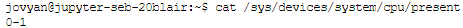
\includegraphics[width=1\textwidth]{images/cpu_cores.PNG}
    \caption{Ouput of the command on line 35}
    \label{fig:cpu_cores}
    \end{figure}
    \end{itemize}
\end{document} 
